\chapter{Progettazione}

La fase di progettazione ha avuto l'obiettivo di tradurre i requisiti individuati
nei capitoli precedenti in un'architettura scalabile, accessibile e coerente con
l'identità aziendale. In questa sezione vengono presentate le decisioni
architetturali chiave, il processo metodologico adottato e l'organizzazione
dell'ecosistema di landing pages.

\section{Decisioni architetturali}
Il punto di partenza era una landing page unica, insufficiente per comunicare i
diversi verticali aziendali e raccogliere dati utili a livello di marketing. La
progettazione ha quindi introdotto tre scelte fondamentali:

\begin{itemize}
  \item \textbf{Architettura multi-landing}: adozione di un monorepo Next.js con sei landing pages dedicate per i verticali aziendali (/it/home, /it/tech-recruiting/, 
/it/ai-adoption/, /it/ai-engineering/, /it/tech-media-agency/, /it/jobs/). Il sistema 
include inoltre pagine preesistenti come blog tecnico e pagina contatti, 
re-integrate nell'architettura unificata. Questa struttura garantisce posizionamento 
SEO ottimale, riuso di componenti comuni e semplicità di manutenzione.
  
  \item \textbf{Strategia di rendering ibrida}: il sistema combina tre approcci 
differenziati per tipo di contenuto. Le 6 landing pages principali dei verticali 
aziendali utilizzano Server-Side Rendering (SSR) on-demand per garantire contenuti 
i18n dinamici e HTML completo per crawler. Il blog preesistente, re-integrato nel 
monorepo, implementa Static Site Generation (SSG) con pre-generazione degli slug 
degli articoli in fase di build. Le chiamate API al backend Django adottano 
Incremental Static Regeneration (ISR) con revalidation a 1 ora, implementando 
pattern Stale-While-Revalidate per ridurre dipendenze da uptime backend. CloudFront 
CDN distribuisce asset statici globalmente, mentre next/image ottimizza 
automaticamente immagini con lazy loading e conversione WebP. Questa architettura 
bilancia SEO (HTML completo server-side), performance (cache CDN), e flessibilità 
contenuti multilingua.
  
  \item \textbf{Design system condiviso}: definizione di una libreria di componenti 
  accessibili basata su ShadCN UI (Radix UI primitives) e Tailwind CSS, costruita 
  su linee guida visive aziendali. Garantisce accessibilità WCAG 2.1 AA nativa, 
  customizzazione completa e riutilizzo del codice UI tra le landing.
\end{itemize}

\section{Metodologia di progettazione e collaborazione} 
Il progetto di redesign è stato organizzato come una \textbf{macro-release trimestrale},
considerata strategica per l'azienda. La fase di progettazione non si è limitata
alla definizione di scelte tecniche, ma ha previsto un percorso strutturato di
analisi, collaborazione e validazione:

\begin{itemize}
  \item \textbf{Analisi iniziale}: revisione delle soluzioni esistenti e
  identificazione dei pattern da mantenere o eliminare.
  \item \textbf{Collaborazione interfunzionale}: raccolta dei requisiti in
  incontri con i team di prodotto, marketing e design, così da garantire
  allineamento tra esigenze di business e soluzioni tecniche.
  \item \textbf{Iterazioni e feedback}: rilascio preliminare delle nuove landing
  a un gruppo ristretto di stakeholder interni, con raccolta feedback e successive
  ottimizzazioni.
  \item \textbf{Approccio Agile}: gestione del lavoro in sprint bisettimanali,
  con daily standup, retrospettive e momenti di confronto dedicati alla revisione
  della qualità.
  \item \textbf{Progettazione responsive}: attenzione fin dall'inizio alle tre
  principali dimensioni di visualizzazione (desktop, tablet e mobile), per
  garantire una user experience coerente e ottimizzata.
\end{itemize}

Questa metodologia ha consentito di ridurre i rischi, migliorare la qualità
finale e assicurare che le landing rispondessero realmente ai bisogni degli utenti
e dell'azienda.

\section{Processo di design e design system}
Il design system è stato sviluppato in stretta collaborazione con il team UX/UI,
a partire da wireframe validati con il product team fino a mockup
high-fidelity realizzati in Figma. Il processo ha incluso:

\begin{itemize}
  \item definizione di design tokens comuni (colori, tipografia, spaziatura),
  condivisi tra Figma e configurazioni Tailwind CSS di progetto;
  \item creazione di componenti modulari con varianti responsive, per garantire 
consistenza visiva e riutilizzo tra le 6 landing pages principali;
\end{itemize}

L'architettura componenti ha permesso di standardizzare elementi ricorrenti garantendo il riutilizzo di molto del codice UI tra le diverse landing.

Questo approccio ha permesso di ridurre i tempi di sviluppo, garantire coerenza tra design e implementazione e abilitare una rapida iterazione.

\begin{figure}[h!]
    \centering
    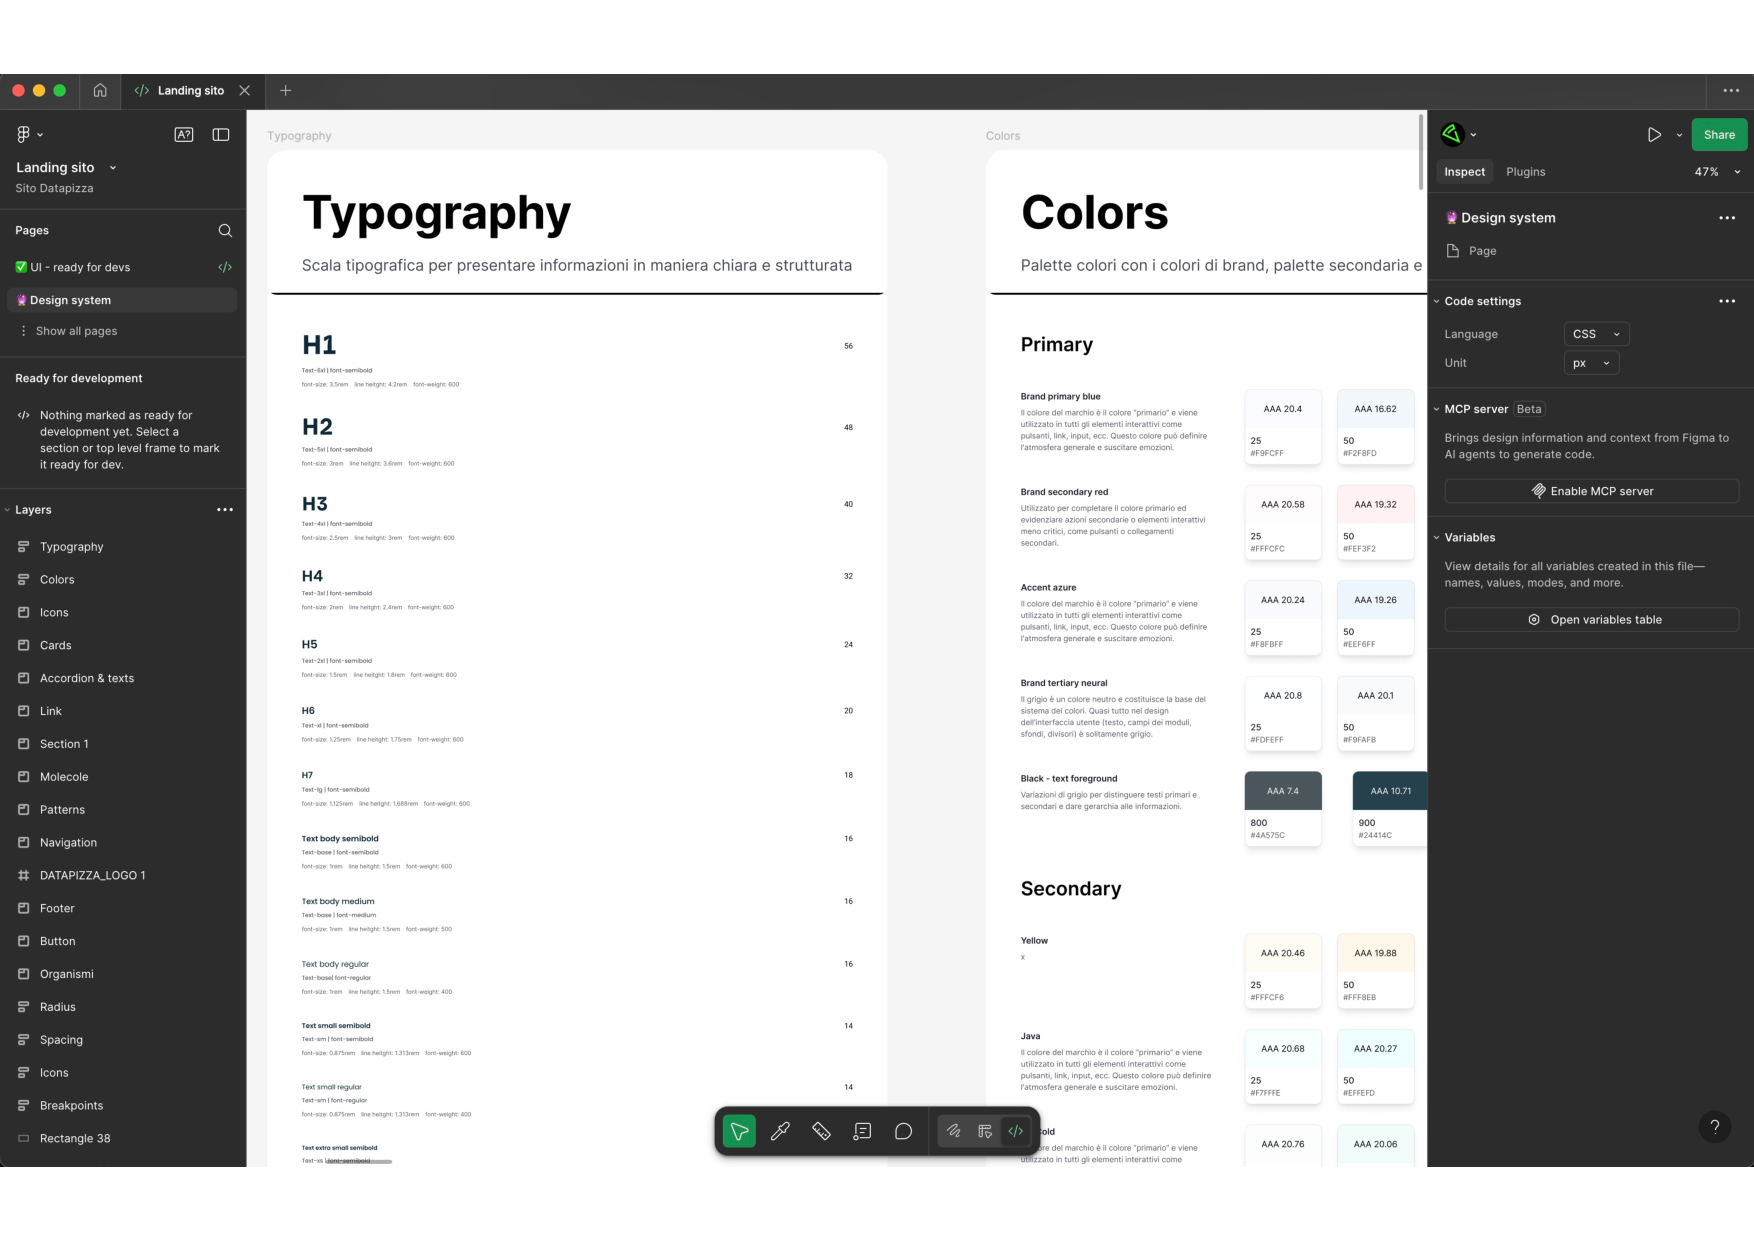
\includegraphics[width=\textwidth]{chapters/figures/design-system.pdf}
    \caption{Esempi di componenti principali del design system.}
    \label{fig:design-system}
\end{figure}

\section{Architettura delle landing pages}
L'ecosistema è stato progettato con una struttura comune di base (\textit{navbar}, 
\textit{footer}) e con personalizzazioni specifiche per ciascun verticale. 
Ogni landing è stata progettata con registro linguistico e UX mirati per target 
specifici:

\begin{itemize}
  \item \textbf{Home Page} (/it/): pagina principale con panoramica generale 
  dei 4 verticali e routing intelligente verso servizi specifici. Target: 
  visitatori generici.
  
  \item \textbf{Tech Recruiting} (/it/tech-recruiting/): registro linguistico 
  consulenziale business-to-business (B2B), layout pulito, form di contatto 
  avanzati con campi aziendali, CTA orientate a demo (``Richiedi demo'', 
  ``Contatta team''). Target: aziende in cerca di talenti tech.
  
  \item \textbf{Tech Community} (/it/tech-media-agency/): linguaggio informale, 
  elementi visuali orientati alla cultura developer, CTA engagement per newsletter 
  ``Commit'', social proof con 500k+ iscritti. Target: developer e tech enthusiast.
  
  \item \textbf{AI Adoption} (/it/ai-adoption/): registro linguistico professionale 
  B2B enterprise, focus upskilling organizzativo e trasformazione interna, case 
  studies aziendali, CTA consulenza personalizzata. Target: HR e management.
  
  \item \textbf{AI Engineering} (/it/ai-engineering/): showcase framework 
  proprietario ``Datapizza AI'' con gallery progetti (Copiloti Sales/HR/Legal/Customer), 
  CTA demo tecnica. Target: CTO e IT Decision Makers.
  
  \item \textbf{Jobs Platform} (/jobs/): stile diretto e colorato 
  business-to-consumer (B2C), call-to-action immediate (``Cerca lavoro'', 
  ``Candidati ora''), esperienza mobile-first, trasparenza salary con RAL sempre 
  visibile, Tech Buddy matching e zero ghosting policy. Target: candidati in cerca 
  di opportunità tech.
\end{itemize}

\begin{figure}[h!]
    \centering
    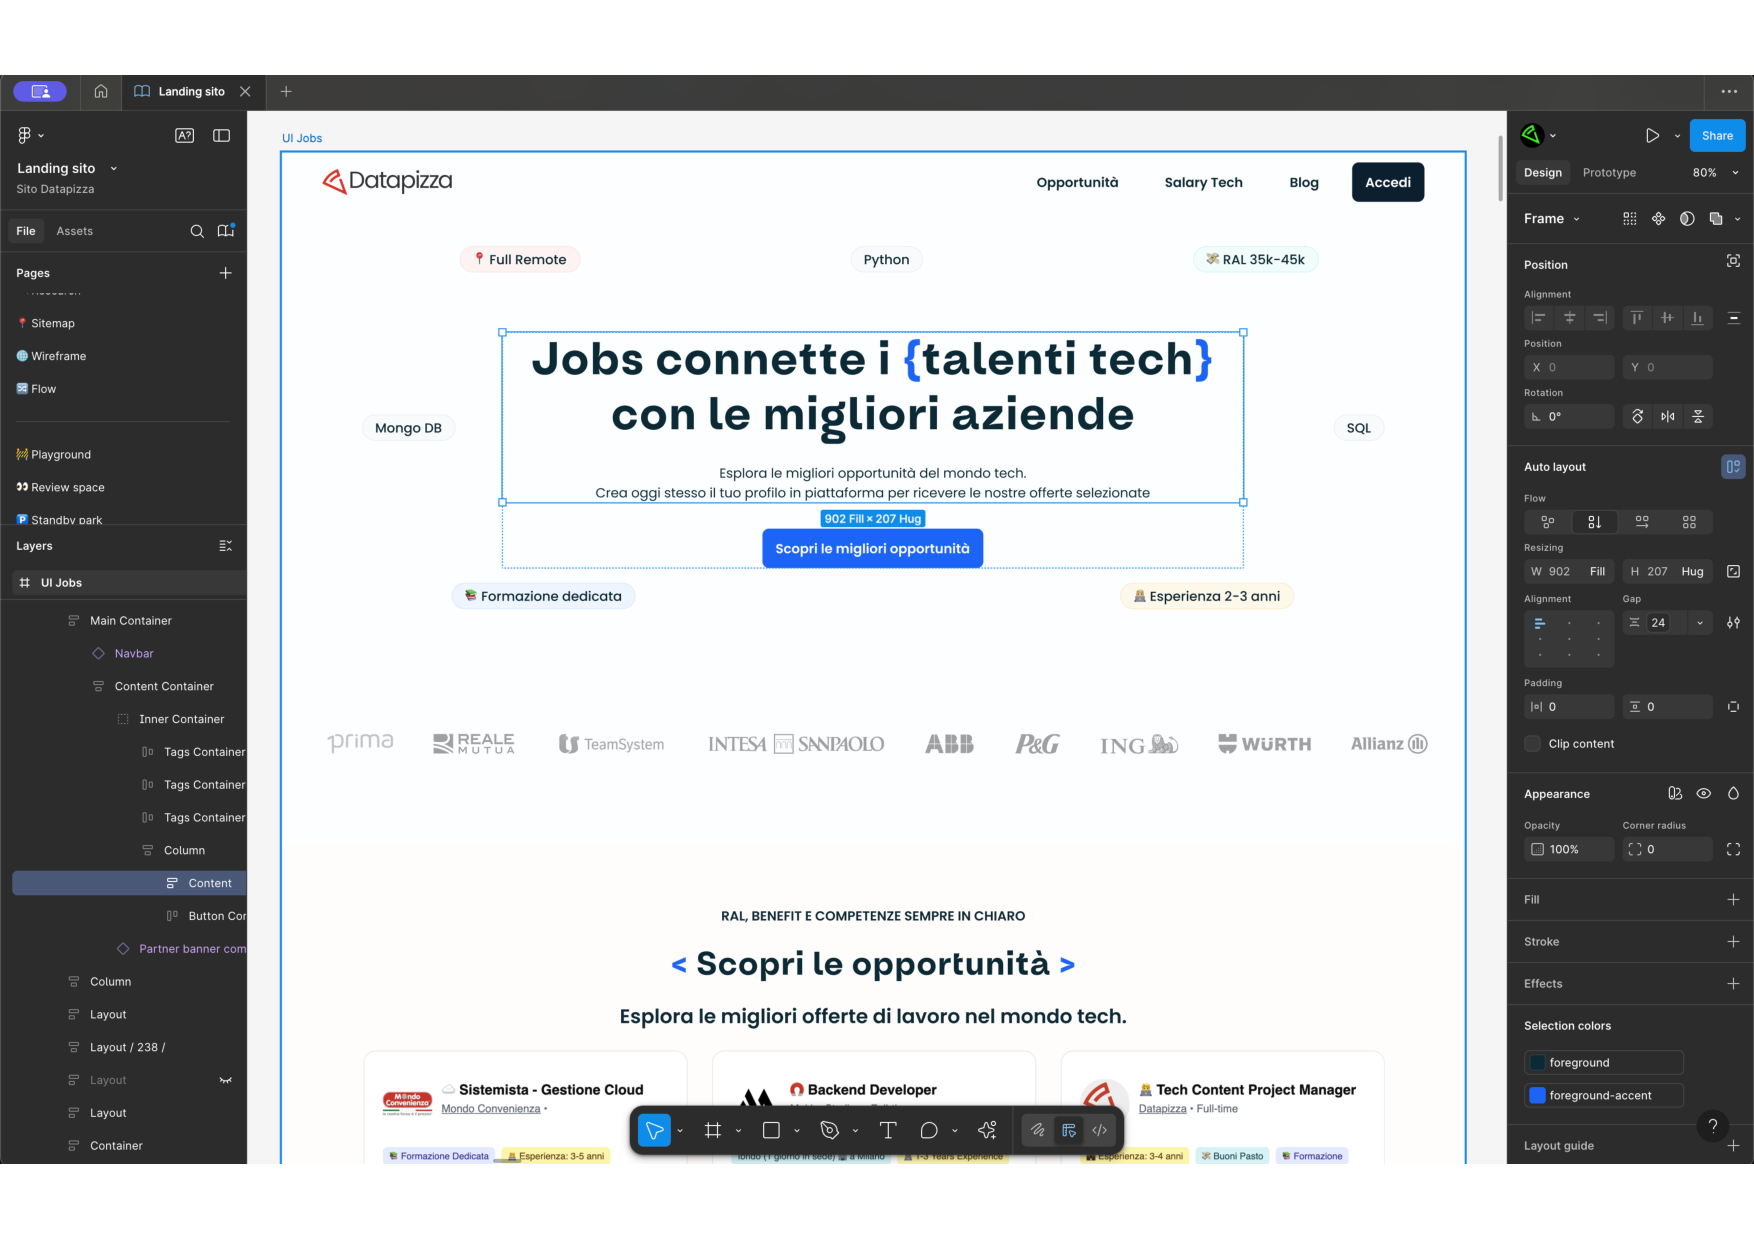
\includegraphics[width=1.1\textwidth]{chapters/figures/mockup.pdf}
    \caption{Mockup desktop della Jobs Platform.}
    \label{fig:jobs-desktop}
\end{figure}

\begin{figure}[h!]
    \centering
    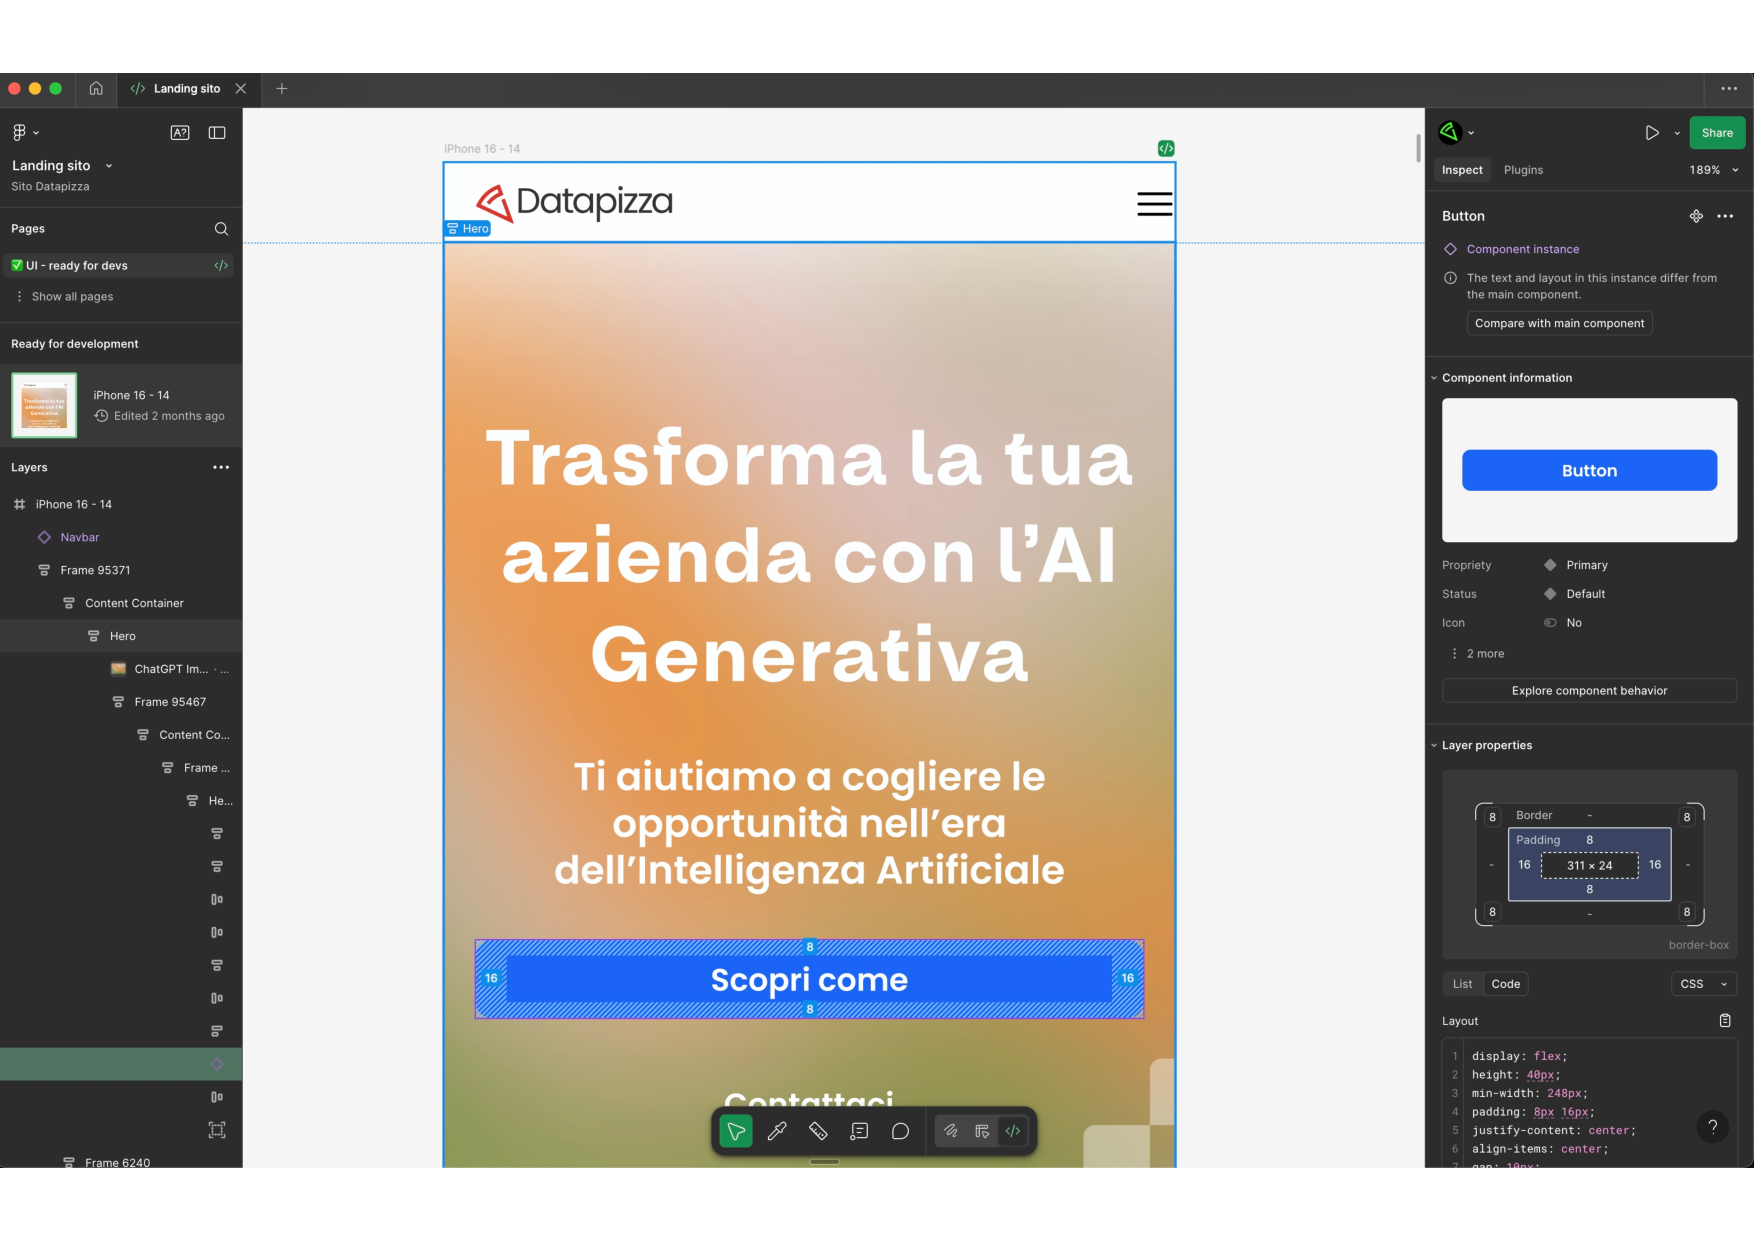
\includegraphics[width=1.1\textwidth]{chapters/figures/mockup2.pdf}
    \caption{Mockup mobile della landing AI Engineering.}
    \label{fig:ai-eng-mobile}
\end{figure}

\section{Tracking e misurabilità}
Il sistema di tracking è stato progettato per migliorare l'implementazione 
precedentemente presente, supportando funnel di conversione specifici per ogni 
verticale. L'integrazione con Mixpanel consente di tracciare page view, 
interazioni e conversioni con granularità maggiore rispetto alla soluzione unica 
precedente.

\subsection{Event taxonomy e funnel}
L'architettura tracking implementa una tassonomia strutturata di eventi:
\begin{itemize}
  \item \textbf{Page events}: page\_view, landing\_loaded
  \item \textbf{Interaction events}: cta\_clicked, scroll\_depth, section\_viewed
  \item \textbf{Conversion events}: form\_submitted, newsletter\_signup
\end{itemize}

Il tracking permette di analizzare funnel di conversione differenziati per verticale:
\begin{itemize}
  \item \textbf{B2B}: landing\_view $\rightarrow$ cta\_click $\rightarrow$ form\_view $\rightarrow$ form\_submit
  \item \textbf{B2C Jobs}: landing\_view $\rightarrow$ search\_used $\rightarrow$ position\_click $\rightarrow$ application\_start
  \item \textbf{Community}: landing\_view $\rightarrow$ scroll\_50\% $\rightarrow$ newsletter\_click $\rightarrow$ newsletter\_submit
\end{itemize}

Questa segmentazione consente analisi specifiche per ottimizzazione delle 
conversioni e identificazione dei punti di drop-off nel customer journey.

\subsection{GDPR compliance}
Particolare attenzione è stata data alla conformità normativa europea con 
approccio privacy-by-design: consenso esplicito tramite cookie banner prima 
di inizializzazione Mixpanel, anonimizzazione automatica degli indirizzi IP 
e gestione opt-out utente.

\bigskip
In sintesi, la progettazione ha permesso di definire una base solida dal punto di
vista tecnico e metodologico, con decisioni architetturali motivate e framework 
scalabile, che ha guidato lo sviluppo e il dispiegamento presentati nei capitoli 
successivi.